\AtBeginDocument{%
%\begin{textblock*}{5.625in}(-50pt,50pt)
%\end{textblock*}
\begingroup\pagestyle{empty}\raggedleft\parindent0pt
\titulagemfront{}
\begin{textblock*}{5.625in}(-100pt,50pt)
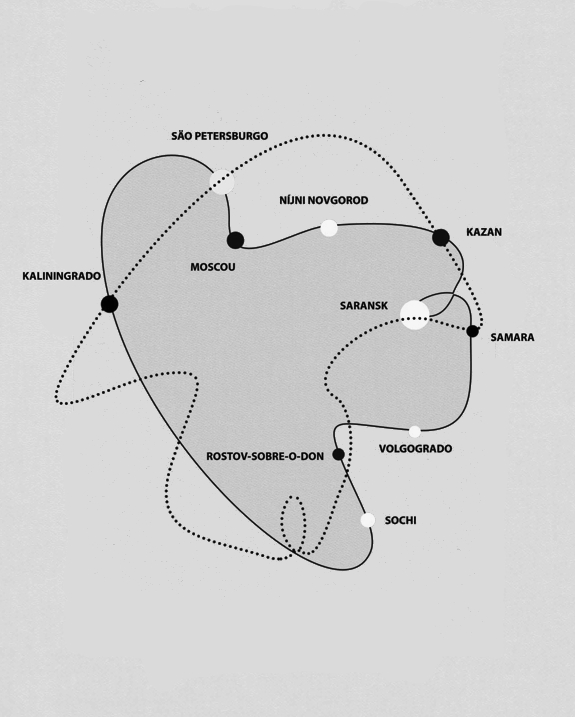
\includegraphics[width=120mm]{./imgs/mapa.jpg}
\end{textblock*}
\vfill
\clearpage

%% Créditos ------------------------------------------------------
\raggedright
\linha{copyright}{\copyrightlivro}
\linhalayout{edição brasileira©}{Hedra \ifdef{\ano}{\ano}{\the\year}}
\linha{tradução©}{\copyrighttraducao}
\linha{organização©}{\copyrightorganizacao}
\linha{introdução©}{\copyrightintroducao}
\linha{ilustração©}{\copyrightilustracao}\smallskip
\linha{título original}{\titulooriginal}
\linha{edição consultada}{\edicaoconsultada}
\linha{primeira edição}{\primeiraedicao}
\linha{agradecimentos}{\agradecimentos}
\linha{indicação}{\indicacao}
\linha{edição}{\edicao}
\linha{coedição}{\coedicao}
\linha{assistência editorial}{\assistencia}
\linha{preparação}{\preparacao}
\linha{revisão}{\revisao}
\linha{iconografia}{\iconografia}
\linha{capa}{\capa}
\linha{imagem da capa}{\imagemcapa}
\linha{ISBN}{\ISBN}
\linha{eISBN}{\eISBN}\smallskip
\begingroup\tiny
\ifdef{\conselho}{\conselho}{\relax}
\par\endgroup\bigskip

\begingroup \tiny

\textit{Grafia atualizada segundo o Acordo Ortográfico da Língua\\
Portuguesa de 1990, em vigor no Brasil desde 2009.}\\


\vfill\textit{Direitos reservados em l\'ingua\\ portuguesa somente para o Brasil}\\\medskip

%
\textsc{editora hedra ltda.}\\
R.~Fradique Coutinho, 1.139 (subsolo)\\
05416-011, São Paulo-\textsc{sp}, Brasil\\
Telefone/Fax +55 11 3097 8304\\\smallskip
editora@hedra.com.br\\
www.hedra.com.br\\
\bigskip
Foi feito o depósito legal.\\\endgroup
\pagebreak\raggedleft
%% Front ---------------------------------------------------------
% Titulo
\titulagem

{\Large \autor \par\vspace{1.5ex}}
\ifdef{\apresentador}{{\small {\apresentador} (\textit{apresentação})} \par}{}
\ifdef{\prefacio}{{\small {\prefacio} (\textit{prefácio})} \par}{}
\ifdef{\organizador}{{\small {\organizador} (\textit{organização})} \par}{}
\ifdef{\introdutor}{{\small {\introdutor} (\textit{introdução})} \par}{}
\ifdef{\tradutor}{{\small {\tradutor} (\textit{tradução})}\par}{}\vspace{1.5cm}

{{\footnotesize{} \ifdef{\numeroedicao}{\numeroedicao}{1}ª edição} \par}

%logos
\vfill
\ifdef{\logo}{\IfFileExists{\logo}{\hfill\includegraphics[width=3cm]{\logo}\hfill\logoum{}\\ São Paulo\_\the\year}}{\logoum\break{} São Paulo\_\the\year}
%\includegraphics[width=.4\textwidth,trim=0 0 25 0]{logo.jpg}\\\smallskip
\par\clearpage\endgroup
% Resumo -------------------------------------------------------
\begingroup \footnotesize \parindent0pt \parskip 5pt \thispagestyle{empty} \vspace*{.25\textheight}\mbox{} \vfill
\baselineskip=.92\baselineskip
\IfFileExists{PRETAS.tex}{\begin{itemize}


\item \textbf{Michel Temer e o fascismo comum} completa a trilogia em que Tales Ab'Sáber disseca
os processos políticos que perpassaram os mandatos dos três últimos presidentes -- Lula, Dilma
Rousseff e Michel Temer, cada qual em um volume --, com enfoque sobretudo nas mentalidades
alicerçadoras desses mesmos processos -- a ``gestão psíquica do poder''.
Nesta terceira publicação, o autor reflete sobre como a onda liberalizante de desmonte das
conquistas sociais promovida pelo governo Temer está
intimamente relacionada à promoção do ódio e da violência, um fascismo
``comum'', porque associado ao cotidiano e às práticas ordinárias, que entorpece a visão
e cria uma paranoia macartista, onde os comunistas do passado são todos os que
vão de encontro a esse liberalismo às avessas.
  
\item \textbf{Tales Ab’Sáber}, psicanalista e ensaísta, é professor de Filosofia da Psicanálise da Universidade Federal 
de São Paulo (\textsc{unifesp}), autor de 
\emph{Lulismo, carisma pop e cultura anticrítica},
\textit{O~sonhar
restaurado: formas do sonhar em Bion, Winnicott e Freud} e
\textit{A música do tempo infinito}. 

\end{itemize}

}{% 
\ifdef{\resumo}{\resumo\par}{}
\ifdef{\sobreobra}{\sobreobra}{}
\ifdef{\sobreautor}{\mbox{}\vspace{4pt}\newline\sobreautor}{}
\ifdef{\sobretradutor}{\newline\sobretradutor}{\relax}
\ifdef{\sobreorganizador}{\vspace{4pt}\newline\sobreorganizador}{\relax}\par}
\thispagestyle{empty} \endgroup
\ifdefvoid{\sobreautor}{}{\pagebreak\ifodd\thepage\paginabranca\fi}
% Sumário -------------------------------------------------------

\sumario{}
\IfFileExists{INTRO.tex}{\include{INTRO}}

\IfFileExists{TEXTO.tex}{\mbox{}\include{TEXTO}}
%\part[{{\def\break{}\titulo}}]{\titulo}
} % fim do AtBeginDocument

% Finais -------------------------------------------------------
\AtEndDocument{%
  \publicidade

\pagebreak\ifodd\thepage\paginabranca\fi

\ifdef{\imagemficha}{\IfFileExists{\imagemficha}{\includegraphics[width=.7\textwidth]{\imagemficha}\par}}{}

\mbox{}\vfill\small\thispagestyle{empty}
\begin{center}
\begin{minipage}{.8\textwidth}
\centering\tiny\noindent{}Adverte-se aos curiosos que se imprimiu este livro \ifdef{\grafica}{na gráfica \grafica}{em nossas oficinas}, 
em \today \ifdef{\papelmiolo}{em papel \papelmiolo}, em tipologia \tipopadrao{}, com diversos sofwares livres, 
entre eles, Lua\LaTeX, git \& ruby. \ifdef{\RevisionInfo{}}{\par(v.\,\RevisionInfo)}{}\par \begin{center}\normalsize\adforn{64}\end{center}
\end{minipage}
\end{center}
}
